%% Direttive TeXworks:
% !TeX root = ./report.tex
% !TEX encoding = UTF-8 Unicode
% !TEX program = arara
% !TEX TS-program = arara
% !TeX spellcheck = it-IT

% arara: pdflatex: { synctex: yes, shell: yes }
% arara: pdflatex: { synctex: yes, shell: yes }

%% Genera un file report.xmpdata con i dati di titolo e autore per il formato PDF/A %%
\begin{filecontents*}{\jobname.xmpdata}
  \Title{Laboratorio~di~Sistemi~Software~--~Tema~finale}
  \Author{Niccolò Maltoni}
  \Copyright{Questo documento è fornito sotto licenza Creative Commons Attribution-ShareAlike 4.0 International}
  \CopyrightURL{http://creativecommons.org/licenses/by-sa/4.0}
\end{filecontents*}

\documentclass{llncs}           % LaTeX document class for Lecture Notes in Computer Science

%%%%%%%%%%%%%%%%%%%%%%%%%%%%%%%%%%%%%%%%%%%%%%%%%%%%%%%%%%%
%% package sillabazione italiana e uso lettere accentate
\usepackage[T1]{fontenc}        % serve per impostare la codifica di output del font
\usepackage{textcomp}           % serve per fornire supporto ai Text Companion fonts
\usepackage[utf8]{inputenc}     % serve per impostare la codifica di input del font
\usepackage[
  english,            % utilizza l'inglese come lingua secondaria
  italian             % utilizza l'italiano come lingua primaria
]{%
  babel,                      % serve per scrivere Indice, Capitolo, etc in Italiano
  varioref                    % introduce il comando \vref da usarsi nello stesso modo del comune \ref per i riferimenti
}
\usepackage{lmodern}            % carica una variante Latin Modern prodotto dal GUST
\usepackage[%
    strict,             % rende tutti gli warning degli errori
    autostyle,          % imposta lo stile in base al linguaggio specificato in babel
    english=american,   % imposta lo stile per l'inglese
    italian=guillemets  % imposta lo stile per l'italiano
]{csquotes}                     % serve a impostare lo stile delle virgolette
%%%%%%%%%%%%%%%%%%%%%%%%%%%%%%%%%%%%%%%%%%%%%%%%%%%%%%%%%%%%%

\usepackage{relsize, etoolbox}  % permette di riferirsi ad ambienti specifici
\AtBeginEnvironment{foreigndisplayquote}{\smaller}

\usepackage{indentfirst}        % serve per avere l'indentazione nel primo paragrafo
\usepackage{url}
\usepackage{setspace}           % serve a fornire comandi di interlinea standard
\usepackage{xspace}

\makeatletter

%%%%%%%%%%%%%%%%%%%%%%%%%%%%%% User specified LaTeX commands.
\usepackage{manifest}

\makeatother

\usepackage{ifpdf}
\usepackage{xcolor}             % serve per la gestione dei colori nel testo

%%%%%%%%%%%%%%%
\ifpdf{}
  \usepackage[pdftex]{graphicx} % serve per includere immagini e grafici
\else
  \usepackage{graphicx}         % serve per includere immagini e grafici
\fi
%%%%%%%%%%%%%%%
\ifpdf{}
  \DeclareGraphicsExtensions{.pdf, .jpg, .tif, .png} % chktex 26
\else
  \DeclareGraphicsExtensions{.eps, .jpg, .png} % chktex 26
\fi
%%%%%%%%%%%%%%%
\usepackage{float}
\usepackage{graphviz}

\usepackage{listings}
\usepackage{listingsutf8}

\definecolor{dkgreen}{rgb}{0,0.6,0}
\definecolor{gray}{rgb}{0.5,0.5,0.5}
\definecolor{mauve}{rgb}{0.58,0,0.82}

\lstset{
  extendedchars=true,
  inputencoding=utf8/latin1,
  frame=single,
  captionpos=b,
  language=Java,
  showspaces=false,
  showtabs=false,
  showstringspaces=false,
  columns=flexible,
  basicstyle={\small\ttfamily},
  numbers=none,
  numberstyle=\tiny\color{gray},
  keywordstyle=\color{blue},
  commentstyle=\color{dkgreen},
  stringstyle=\color{mauve},
  breaklines=true,
  breakatwhitespace=true,
  keepspaces=true,
  numbersep=5pt,
  tabsize=2
}

\lstdefinelanguage{qa}{
  basicstyle=\ttfamily\scriptsize,
  numbers=left,
  numberstyle=\scriptsize,
  stepnumber=1,
  numbersep=8pt,
  tabsize=2,
  showstringspaces=false,
  breaklines=true,
  breakatwhitespace=true,
  keywordstyle=\color{mauve}\bfseries,
  commentstyle=\color{dkgreen},stringstyle=\color{blue},
  morekeywords={System,Event,Dispatch,Context,QActor,Rules,State,%
      demo,whenMsg,whenEvent,onMsg,onEvent,transition,stopAfter,%
      whenTime,resumeLastPlan,initial,finally,javaRun,println,%
      emit,forward,do},
  otherkeywords={:,->,-m,;,.,\,,[,],:-},
  morestring=*[d]{``}, % chk segnala errore con "
  morecomment=[l]{//},
  morecomment=[s]{/*}{*/} % chk segnala errore con \/* e con *\/
}

\newcommand{\java}{\textsf{Java}}
\newcommand{\contact}{\emph{Contact}}
\newcommand{\corecl}{\texttt{corecl}}
\newcommand{\medcl}{\texttt{medcl}}
\newcommand{\msgcl}{\texttt{msgcl}}
\newcommand{\android}{\texttt{Android}}
\newcommand{\dsl}{\texttt{DSL}}
\newcommand{\jazz}{\texttt{Jazz}}
\newcommand{\rtc}{\texttt{RTC}}
\newcommand{\ide}{\texttt{Contact-ide}}
\newcommand{\xtext}{\texttt{XText}}
\newcommand{\xpand}{\texttt{Xpand}}
\newcommand{\xtend}{\texttt{Xtend}}
\newcommand{\pojo}{\texttt{POJO}}
\newcommand{\junit}{\texttt{JUnit}}

\newcommand{\action}[1]{\texttt{#1}\xspace}
\newcommand{\code}[1]{{\small{\texttt{#1}}}\xspace}
\newcommand{\codescript}[1]{{\scriptsize{\texttt{#1}}}\xspace}

\newcommand{\requirement}[1]{\hypertarget{req:#1}{\textcolor{blue}{#1}}}
\newcommand{\requirementref}[1]{\hyperlink{req:#1}{\textcolor{blue}{#1}}}

% Cross-referencing
\newcommand{\labelsec}[1]{\label{sec:#1}}
\newcommand{\xs}[1]{\sectionname~\ref{sec:#1}}
\newcommand{\xsp}[1]{\sectionname~\ref{sec:#1} \onpagename~\pageref{sec:#1}}
\newcommand{\labelssec}[1]{\label{ssec:#1}}
\newcommand{\xss}[1]{\subsectionname~\ref{ssec:#1}}
\newcommand{\xssp}[1]{\subsectionname~\ref{ssec:#1} \onpagename~\pageref{ssec:#1}}
\newcommand{\labelsssec}[1]{\label{sssec:#1}}
\newcommand{\xsss}[1]{\subsectionname~\ref{sssec:#1}}
\newcommand{\xsssp}[1]{\subsectionname~\ref{sssec:#1} \onpagename~\pageref{sssec:#1}}
\newcommand{\labelfig}[1]{\label{fig:#1}}
\newcommand{\xf}[1]{\figurename~\ref{fig:#1}}
\newcommand{\xfp}[1]{\figurename~\ref{fig:#1} \onpagename~\pageref{fig:#1}}
\newcommand{\labeltab}[1]{\label{tab:#1}}
\newcommand{\xt}[1]{\tablename~\ref{tab:#1}}
\newcommand{\xtp}[1]{\tablename~\ref{tab:#1} \onpagename~\pageref{tab:#1}}
% Category Names
\newcommand{\sectionname}{Section}
\newcommand{\subsectionname}{Subsection}
\newcommand{\sectionsname}{Sections}
\newcommand{\subsectionsname}{Subsections}
\newcommand{\secname}{\sectionname}
\newcommand{\ssecname}{\subsectionname}
\newcommand{\secsname}{\sectionsname}
\newcommand{\ssecsname}{\subsectionsname}
\newcommand{\onpagename}{on page}

\newcommand{\xauthA}{Niccolò~Maltoni}
\newcommand{\xfaculty}{II~Faculty~of~Engineering}
\newcommand{\xunibo}{Alma~Mater~Studiorum~--~University~of~Bologna}

\usepackage{enumitem}

\setcounter{secnumdepth}{2}   % Numera fino alla sottosezione nel corpo del testo
\setcounter{tocdepth}{3}      % Numera fino alla sotto-sottosezione nell'indice

\usepackage[%
  depth=3,              % equivale a bookmarksdepth di hyperref
  open=false,           % equivale a bookmarksopen di hyperref
  numbered=true         % equivale a bookmarksnumbered di hyperref
]{bookmark}                     % Gestisce i segnalibri meglio di hyperref
\usepackage{hyperref}           % Gestisce tutte le cose ipertestuali del pdf
\hypersetup{%
  pdfpagemode={UseNone},
  hidelinks,            % nasconde i collegamenti (non vengono quadrettati)
  hypertexnames=false,
  linktoc=all,          % inserisce i link nell'indice
  unicode=true,         % only Latin characters in Acrobat’s bookmarks
  pdftoolbar=false,     % show Acrobat’s toolbar?
  pdfmenubar=false,     % show Acrobat’s menu?
  plainpages=false,
  breaklinks,
  pdfstartview={Fit},
  pdfauthor={Niccolò Maltoni},
  pdfcreator={Niccolò Maltoni},
  pdftitle={Laboratorio di Sistemi Software - Tema finale}, % chktex 8
  pdflang={it}
}

\usepackage[a-1b]{pdfx}
\usepackage[%
  italian,            % definizione delle lingue da usare
  nameinlink          % inserisce i link nei riferimenti
]{cleveref}                     % permette di usare riferimenti migliori dei \ref e dei varioref

\begin{document}

\title{\textbf{LSS --- Laboratorio di Sistemi Software}\\tema finale\\\textit{\small \url{https://github.com/NiccoMlt/ISS-2018-Final-Task}}}

\author{\xauthA}

\institute{%
  \xunibo{}\\\email{}\ \href{mailto:niccolo.maltoni@studio.unibo.it}{niccolo.maltoni@studio.unibo.it}
}

{\def\addcontentsline#1#2#3{}\maketitle}

\tableofcontents

%===========================================================================
\section{Introduzione}\labelsec{intro}
%% Direttive TeXworks:
% !TeX root = ../report.tex
% !TEX encoding = UTF-8 Unicode
% !TEX program = arara
% !TEX TS-program = arara
% !TeX spellcheck = it-IT

% arara: pdflatex: { synctex: yes, shell: yes, interaction: nonstopmode }
% arara: pdflatex: { synctex: yes, shell: yes, interaction: nonstopmode }

Per realizzare il task finale proposto, la software house si propone di utilizzare una metodologia agile \textit{Scrum-like}
seguendo un approccio \textit{top-down} \textit{model-driven};
il lavoro sarà dunque diviso in Sprint successivi al termine di ognuno dei quali verrà compiuta una \textit{Sprint Review}
con il committente, il quale potrà suggerire correzioni e nuovi requisiti.
Di conseguenza, al termine di ogni Sprint l'obiettivo sarà di consegnare al cliente un prodotto di valore (\textit{valuable}),
per quanto non completo in tutte le sue parti.

In ogni Sprint verranno eseguite tutte le fasi di un processo di sviluppo software, affinando progressivamente il risultato,
migliorando il prodotto esistente e affrontando le problematiche non ancora analizzate;
lo sviluppo procederà dunque con un approccio incrementale e un'andatura monotona crescente, promuovendo da un lato
l'\textit{estendibilità} e il \textit{cambiamento}, senza però impattare pesantemente il prodotto già consegnato.

Per ogni Sprint, dunque, si procederà per fasi:
la prima fase sarà un'attenta \textbf{analisi dei requisiti}, con l'obiettivo di di identificare con chiarezza
tutti i requisiti del sistema, tracciandoli in maniera univoca e identificando le entità in gioco.
Successivamente, è importante effettuare un'\textbf{analisi del problema}, nella quale verranno sviscerate tutte le problematiche
relative alla progettazione del sistema (senza però scendere in dettagli implementativi),
rimanendo \textit{technology-independent} pur essendo \textit{technology-aware}.
Definita un'architettura logica, si procede con la \textbf{progettazione} e con il \textbf{test planning}.

%===========================================================================

%===========================================================================
% \section{Visione}\labelsec{vision}
% TODO: sezione probabilmente non necessaria
%===========================================================================

%===========================================================================
% \section{Obiettivi}\labelsec{goals}
% TODO: sezione probabilmente non necessaria
%===========================================================================

%===========================================================================
\section{Requisiti}\labelsec{requirements}
%% Direttive TeXworks:
% !TeX root = ../report.tex
% !TEX encoding = UTF-8 Unicode
% !TeX spellcheck = it-IT

% arara: pdflatex: { synctex: yes, shell: yes, interaction: nonstopmode }
% arara: bibtex
% arara: pdflatex: { synctex: yes, shell: yes, interaction: nonstopmode }
% arara: pdflatex: { synctex: yes, shell: yes, interaction: nonstopmode }

Di seguito è riportato il documento dei requisiti fornito dal committente:

\begin{foreigndisplayquote}{english}
  A \texttt{ddr} robot (\requirement{discovery}) must be used to check for the existence of a bomb in the hall of a airport.

  The hall has been evacuated, but on its (flat) floor remains the luggage left by the travellers.
  The robot \requirementref{discovery} can be remotely controlled via smart device by an human operator working in a protected area.
  The robot must start its work under the following conditions:

  \begin{itemize}
    \item the \texttt{operator} has sent a \texttt{EXPLORE} command (\requirement{R-startExplore}) by using a \texttt{GUI} interface (\requirement{console}) running on the smart device;
    \item the value of the temperature in the hall is not higher than a prefixed value (\requirement{R-TempOk}): (e.g. 25 degrees Celsius).
  \end{itemize}

  The software system running on the robot and on the operator device must provide the following functionalities:

  \begin{enumerate}
    \item
      the robot must explore (in `autonomous way') the hall (\requirement{R-explore}) with the goal to reach each bag on the hall-floor;
    \item
      during the exploration phase the operator can stop (\requirement{R-stopExplore}) the robot and send to it a command to return to its initial position (\requirement{R-backHome}) or to continue the exploration phase (\requirement{R-continueExplore});
    \item
      while exploring, \requirementref{discovery} must blink a \texttt{Led} put on it (\requirement{R-blinkLed}) and update the operator console with information on the robot/discovery state (\requirement{R-consoleUpdate});
    \item
      when \requirementref{discovery} is in proximity of a bag, it must:
      \begin{itemize}
        \item stop (\requirement{R-stopAtBag});
        \item take a picture (\requirement{R-takePhoto}) of the bag;
        \item send the photo to the operator device (\requirement{R-sendPhoto});
      \end{itemize}
    \item
        when the operator device receives a photo, it executes a tool able to understand if the bag could be a bomb.
        In case of `bomb-detected', the operator device:
        \begin{itemize}
          \item alerts the operator (\requirement{R-alert});
          \item stores the photo (\requirement{R-storePhoto}) on some permanent storage device, together with contextual information (e.g.\ time, robot-position, etc.);
          \item sends to the robot the command to return to its initial position (\requirement{R-backHomeSinceBomb});
        \end{itemize}
        Otherwise, the operator device sends to the robot the command to continue the exploration (\requirement{R-continueExploreAfterPhoto});
    \item
      the operator alerted for a possible bomb:
      \begin{itemize}
        \item waits until the robot is returned to its initial position (\requirement{R-waitForHome});
        \item when \requirementref{discovery} is at home, tells to \hypertarget{ref:retriever}{another robot} (equipped with proper tools) to reach the discovered bag (\requirement{R-reachBag}) in order to put the bag in safe container and transport it to the initial position (\requirement{R-bagAtHome}).
      \end{itemize}
  \end{enumerate}
\end{foreigndisplayquote}

%===========================================================================

%===========================================================================
\section{Analisi dei requisiti generale}\labelsec{req_analysis}
%% Direttive TeXworks:
% !TeX root = ../report.tex
% !TEX encoding = UTF-8 Unicode
% !TEX program = arara
% !TEX TS-program = arara
% !TeX spellcheck = it-IT

% arara: pdflatex: { synctex: yes, shell: yes, interaction: nonstopmode }
% arara: pdflatex: { synctex: yes, shell: yes, interaction: nonstopmode }

Dall'analisi dei requisiti forniti dal committente è possibile definire i seguenti requisiti:

\begin{enumerate}
  \item
    il sistema è distribuito e composto da tre componenti principali:
    \begin{description}
      \item[\textbf{Robot \requirementref{discovery}}] Si intende un componente che esplori (\requirementref{R-explore}) autonomamente l'ambiente seguendo specifici comandi dell'operatore;
      \item[\textbf{Robot \requirementref{retriever}}] Si intende un componente che raggiunga la bomba scoperta e la porti a casa;
      \item[\textbf{Componente \requirementref{console}}] Il componente utilizzato da remoto dall'operatore attraverso un PC od uno smartphone;
    \end{description}

  \item
    gli \textbf{ostacoli} sono \textit{statici} e, dato che viene assunto che la hall sia stata evacuata, possono essere divisi in:
    \begin{itemize}
      \item \textit{muri},
      \item \textit{borse}.
    \end{itemize}

  \item
    il \textbf{robot \requirementref{discovery}} deve iniziare l'esplorazione (\requirementref{R-explore}) solo nel caso in cui la temperatura sia sotto la soglia di 25°C (\requirementref{R-TempOk}) e riceva il comando di esplorazione dalla \textbf{\requirementref{console}} (\requirementref{R-startExplore});

  \item
    il comando \textit{Esplora} (\requirementref{R-startExplore}) viene inviato dalla \textbf{\requirementref{console}} unicamente al \textbf{robot \requirementref{discovery}};

  \item
    le informazioni dello stato del \textbf{robot \requirementref{discovery}} vengono inviate dallo stesso alla \textbf{\requirementref{console}} (\requirementref{R-consoleUpdate});
    \begin{description}
      \item[\textbf{Stato del robot}] Si intendono almeno le sue coordinate e l'azione corrente;
    \end{description}

  \item
    il \textbf{robot \requirementref{discovery}} è equipaggiato con un \textbf{sonar} nella sua parte anteriore per permettergli di individuare eventuali ostacoli (\requirementref{R-stopAtBag}) e di un \textbf{led} che dovrà saper far lampeggiare (\requirementref{R-blinkLed});

  \item
    qualora il \textbf{robot \requirementref{discovery}} incontri un ostacolo, deve:
    \begin{itemize}
      \item fermarsi (\requirementref{R-stopAtBag});
      \item scattare una foto (\requirementref{R-takePhoto});
      \item mandare la foto (\requirementref{R-sendPhoto}) alla \textbf{\requirementref{console}}.
    \end{itemize}
    A sua volta, la \textbf{\requirementref{console}} dovrà:
    \begin{itemize}
      \item allertare l'operatore (\requirementref{R-alert});
      \item salvare la foto (\requirementref{R-storePhoto}) ricevuta con dati di contesto;
      \item mandare il robot a casa (\requirementref{R-backHomeSinceBomb}) o farlo continuare (\requirementref{R-continueExploreAfterPhoto}).
    \end{itemize}

  \item
    il \textbf{robot \requirementref{retriever}} deve conoscere il percorso per raggiungere la bomba (\requirementref{R-reachBag}) una volta che il \textbf{robot \requirementref{discovery}} sarà tornato (\requirementref{R-waitForHome}) e il percorso per tornare con la bomba (\requirementref{R-bagAtHome});

  \item
    il cuore del sistema è la definizione della \textit{business logic} del robot che concerne l'esplorazione autonoma della hall;

  \item
    in qualsiasi momento, anche mentre in esplorazione, il \textbf{robot \requirementref{discovery}} deve essere reattivo ad un comando di halt (\requirementref{R-stopExplore}) inviatogli dalla \textbf{\requirementref{console}}.
\end{enumerate}

Nelle sezioni successive ciascun requisito ed entità verrà analizzato con maggior dettaglio.

\subsection{Componenti identificati}\labelssec{components}

\subsubsection{Console}\labelsssec{console}

La console consiste in un'interfaccia grafica attraverso la quale l'operatore può interagire con il sistema.

Essa permette di interagire con il robot esploratore inviandogli un comando per far partire l'esplorazione.
Attraverso la console l'utente può stoppare l'esplorazione per poi scegliere di continuarla oppure di farlo tornare alla base.
In caso di rilevamento di un ordigno la console deve segnalarlo all'utente, salvare la foto ed inviare al robot il comando per tornare alla posizione iniziale.
Infine, deve consentire l'invio di un comando per far sì che un altro robot possa recuperare l'ordigno.

\subsubsection{Robot Discovery}\labelsssec{discovery}

Robot Discovery è un ddr robot che si occupa dell'esplorazione dell'ambiente per rilevare la presenza di eventuali ordigni.
Il robot per il committente è un dispositivo fisico in grado di muoversi nell'ambiente grazie a delle ruote motrici, fornito di un LED
e dotato di un sonar posto frontalmente per individuare ostacoli.

Esso permette di essere avviato e/o stoppato remotamente.
Deve far lampeggiare un LED ed inviare informazione sullo stato suo e dell'esplorazione.
In prossimità di una valigia deve fermarsi, scattare una foto ed inviarla all'operatore.

\subsubsection{Robot Retriever}\labelsssec{retriever}

Robot Discovery è un drr robot che ha il compito di raggiungere la borsa individuata (contenente la bomba) e trasportarla alla posizione iniziale.

\subsection{Dettaglio sui requisiti della fase di esplorazione}\labelssec{explore}

\begin{description}[itemsep=1em]
  \item[\requirementref{R-explore}]\labelsssec{R-explore}

  Durante la fase di esplorazione il robot deve muoversi nella stanza, raccogliendo informazioni per creare una rappresentazione del territorio comprendente ostacoli e posizioni degli ordigni.
  L'output di questa fase consiste in una rappresentazione che deve riportare le informazioni riguardanti la stanza e deve essere condivisa con gli altri componenti del sistema.
  In questa rappresentazione dovranno essere segnalate le posizioni di eventuali ostacoli, in modo che il robot Retriever possa ottimizzare il proprio percorso verso l'ordigno da rimuovere.

  \item[\requirementref{R-startExplore}]\labelsssec{R-startExplore}

  L'esplorazione deve partire in seguito all'invio di un comando da parte dell'operatore.

  \item[\requirementref{R-TempOk}]\labelsssec{R-TempOk}

  L'esplorazione deve partire solo se la temperatura rispetta le condizioni prestabilite.

  \item[\requirementref{R-stopExplore}]\labelsssec{R-stopExplore}

  L'esplorazione deve stopparsi in caso l'utente lo richieda.
  Emerge quindi la necessità da parte del robot di essere reattivo ai comandi ricevuti.

  \item[\requirementref{R-backHome}]\labelsssec{R-backHome}

  Il robot deve tornare alla posizione iniziale se richiesto dall'utente al seguito dello stop dell'esplorazione.

  \item[\requirementref{R-continueExplore}]\labelsssec{R-continueExplore}

  Il robot deve continuare l'esplorazione se richiesto dall'utente.

  \item[\requirementref{R-blinkLed}]\labelsssec{R-blinkLed}

  Il LED del robot deve lampeggiare se esso è in fase di esplorazione.

  \item[\requirementref{R-consoleUpdate}]\labelsssec{R-consoleUpdate}

  La console deve contenere le informazioni aggiornate riguardo allo stato di esplorazione del robot.

  \item[\requirementref{R-stopAtBag}]\labelsssec{R-stopAtBag}

  Il robot deve fermarsi in prossimità di una valigia.

  \item[\requirementref{R-takePhoto}]\labelsssec{R-takePhoto}

  Il robot deve scattare una fotografia all'ostacolo appena individuato.

  \item[\requirementref{R-sendPhoto}]\labelsssec{R-sendPhoto}

  Il robot deve inviare la fotografia appena scattata alla console.

  \item[\requirementref{R-alert}]\labelsssec{R-alert}

  Il device dell'operatore, una volta ricevuta la foto, deve essere in grado di riconoscere
  se la valigia contiene una bomba, ed, in questo caso, inviare una notifica all'operatore.

  \item[\requirementref{R-storePhoto}]\labelsssec{R-storePhoto}

  La fotografia deve essere salvata in modo permanente contestualmente alle informazioni relative.

  \item[\requirementref{R-backHomeSinceBomb}]\labelsssec{R-backHomeSinceBomb}

  In caso la valigia contenga un ordigno, il robot Discovery deve tornare immediatamente alla posizione iniziale.

  \item[\requirementref{R-continueExploreAfterPhoto}]\labelsssec{R-continueExploreAfterPhoto}

  Se la valigia non contiene una bomba allora al robot viene comandato di continuare l'esplorazione, aggiornando contestualmente la mappa del territorio.
\end{description}

\subsection{Dettaglio sui requisiti della fase di recupero}\labelssec{retrieve}

\begin{description}[itemsep=1em]

  \item[\requirementref{R-waitForHome}]\labelsssec{R-waitForHome}

  Il sistema è in attesa che il robot discovery torni alla base.

  \item[\requirementref{R-reachBag}]\labelsssec{R-reachBag}

  Il robot Retriever deve raggiungere la posizione dell'ordigno.
  L'assunzione fatta è che il territorio sia rimasto invariato rispetto alla fase di esplorazione precedente.

  \item[\requirementref{R-bagAtHome}]\labelsssec{R-bagAtHome}

  Il robot Retriever dopo aver raccolto l'ordigno in un contenitore sicuro deve tornare alla base evitando gli ostacoli come in precedenza.

\end{description}


\section{Sprint 1}\labelsec{sprint1}
%% Direttive TeXworks:
% !TeX root = ../report.tex
% !TEX encoding = UTF-8 Unicode
% !TEX program = arara
% !TEX TS-program = arara
% !TeX spellcheck = it-IT

% arara: pdflatex: { synctex: yes, shell: yes }
% arara: pdflatex: { synctex: yes, shell: yes }

Essendo lo Sprint iniziale, è stata realizzata un'attenta analisi di tutti i requisiti forniti dal committente
con uno sguardo generale su tutto il sistema, in modo da poter chiarire con quest'ultimo eventuali incomprensioni.

L'obiettivo di questo primo Sprint è individuare struttura e interazioni di massima del sistema; in particolare:
\begin{itemize}
  \item
    con l'analisi dei requisiti si vuole far emergere i componenti del sistema del committente;
  \item
    con l'analisi del problema si vuole identificare eventuali ulteriori componenti di interesse per la futura progettazione.
\end{itemize}

Una volta formalizzata un prima analisi dei requisiti generale, reperibile in questo documento alla \Cref{sec:req_analysis},
il passo successivo è individuare i requisiti prioritari da realizzare in questo primo Sprint, in modo da poterli analizzare nel dettaglio.

\subsection{Analisi dei requisiti}\labelssec{sp1:req_analysis}

Dopo aver delineato tutti i requisiti base, si è scelto di approfondire quelli maggiormente fondanti e di valore per il prodotto:

\begin{description}[itemsep=1em]
  \item[\requirementref{R-startExplore}]
    tramite una console grafica l'utente dovrà poter inviare un comando di inizio esplorazione, il comando dovrà essere ricevuto dal robot, il quale dovrà dare inizio alla fase di esplorazione se il requisito successivo è verificato.
  \item[\requirementref{R-explore}]
    l'esplorazione per questo sprint iniziale sarà dummy, in modo da permettere all'utente di vedere il robot muoversi.
  \item[\requirementref{R-tempOk}]
    l'esplorazione dovrà partire soltanto se la temperatura è inferiore ad una certa soglia.
    Da requisiti iniziali non è chiaro se il robot debba essere reattivo a cambi della temperatura durante la fase di esplorazione;
    per il momento si assume di no.
  \item[\requirementref{R-stopExplore}]
    in seguito ad un comando dell'utente l'esplorazione dovrà essere interrotta ed il robot rimarrà in attesa di sapere dall'utente se deve tornare a casa oppure proseguire l'esplorazione appena interrotta.
  \item[\requirementref{R-continueExplore}]
    se l'utente ha inviato il comando per riprendere l'esplorazione il robot deve riprenderla.
  \item[\requirementref{R-backHome}]
    se invece l'utente ha deciso che il robot debba tornare alla sua base, il robot deve farlo.
    Si specifica però che in questo primo sprint non essendo stato ancora introdotto il concetto di mappa, dunque il ritorno a casa sarà soltanto simulato.
\end{description}

Il prodotto dell'analisi dei requisiti deve essere una prima versione dell'architettura logica, che modelli e rappresenti formalmente i requisiti del sistema.

\subsection{Metamodello e QA}\labelssec{qa}

Per rappresentare in maniera formale l'architettura logica, si è scelto di utilizzare il meta-linguaggio QA, nella sua versione \textbf{1.5.13.2}.
Questo linguaggio è stato messo a disposizione dalla software house e permette di superare le limitazioni intrinseche della modellazione UML
(principalmente object-oriented e con notevoli limitazioni nel distribuito).

Il linguaggio QA è adatto per costruire modelli eseguibili di sistemi software e permette di generare rappresentazioni grafiche del sistema,
permettendo di facilitare la comprensione di \textbf{struttura}, \textbf{interazione} e \textbf{comportamento} dello stesso.

\begin{figure}[H]
  \centering
  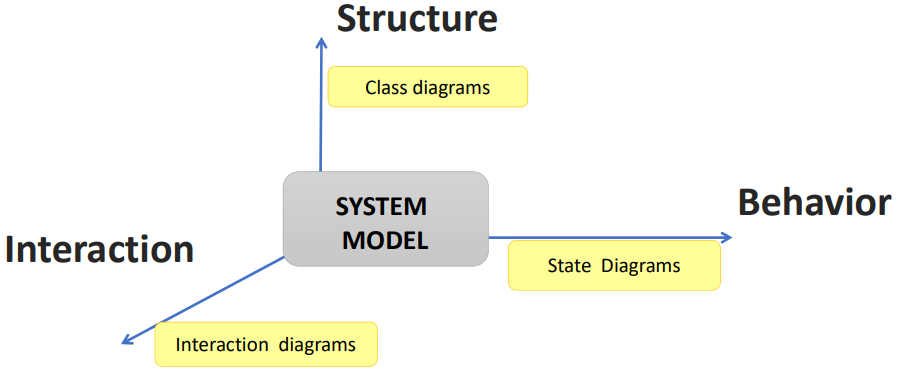
\includegraphics[width=1\textwidth]{res/logicalArchitecture.png}%
  \label{fig:logicalArchitecture}
\end{figure}

\subsection{Architettura logica in output all'analisi dei requisiti}\labelssec{sp1:arch_logica_req}

Partendo con un approccio top-down, sono stati prima di tutto riconosciuti i 3 componenti principali:

\begin{figure}[H]
  \centering
  \includegv[width=1\textwidth]{res/sprint1/requirements/console}%
  \caption{Console}%
  \label{fig:sp1:req:console}
\end{figure}

\begin{figure}[H]
  \centering
  \includegv[width=1\textwidth]{res/sprint1/requirements/robotdiscovery}%
  \caption{Robot Discovery}%
  \label{fig:sp1:req:robotdiscovery}
\end{figure}

\begin{figure}[H]
  \centering
  \includegv[width=1\textwidth]{res/sprint1/requirements/robotretrieval}%
  \caption{Robot Retrieval}%
  \label{fig:sp1:req:robotretrieval}
\end{figure}

Analizzando i tipi di interazioni, si è deciso che queste ultime funzionano come seguono:

\begin{itemize}
  \item
    Il robot invia informazioni sullo stato alla console tramite l'invio di messaggi di tipo \textbf{fire-and-forget}
    (\texttt{dispatch} nel meta-linguaggio QA).

    Essendo il tipo di interazione \textit{uno-ad-uno}, si è ritenuto appropriato utilizzare come metodo di interazione lo scambio di messaggi.

  \item
    La console invia istruzioni ai robot anch'essa tramite l'invio di messaggi;
    le ragioni sono analoghe al caso precedente,
    e a maggior ragione è evidente come vi sia uno e soltanto un destinatario.

\end{itemize}

\clearpage

Di seguito è riportata la prima versione dell'architettura logica in output all'analisi dei requisiti formalizzata tramite metamodello QA\@.

\lstinputlisting[language=qa]{res/sprint1/requirements/robot.qa}

\subsection{Analisi del problema}\labelssec{sp1:prob_analysis}

Durante la fase di analisi del problema si è deciso di dividere il \textbf{robot discovery} in due componenti principali:

\begin{itemize}
  \item uno che conterrà la business logic (\textbf{robot-mind}).
  \item uno che lavorerà come adattatore per i robot in ambiente virtuale o fisico (\textbf{robot-adapter}).
\end{itemize}

Inoltre è stato aggiunto un componente che si occupa di valutare se le condizioni per il funzionamento del robot siano favorevoli o meno e di informare la \textbf{robot-mind}.

\subsubsection{World observer}\labelsssec{sp1:world_observer}

Dato che le informazioni ambientali vengono generate esternamente sia rispetto al robot che rispetto alla console,
è stato ritenuto approriato istruire un nuovo componente nel sistema che si occupi di osservare le variazioni delle condizioni ambientali
e che vada a valutarle per decidere se queste sono favorevoli o meno al corretto funzionamento del robot (\requirementref{R-tempOk});
una volta valutate tali condizioni, il componente emette un evento tramite il quale informa il resto del sistema.

\subsubsection{Robot Adapter e Robot Mind}\labelsssec{sp1:mind_adapter}

Si è ritenuto opportuno separare la logica di funzionamento del robot dal componente che si occupa di eseguire le istruzioni per vari motivi,
tra cui ottenere una maggiore separazione tra un componente chiave contenente la \textbf{business logic}, core del sistema, (\textbf{robot-mind}) ed un mero esecutore di comandi (\textbf{robot-adapter}).
Tra l'altro questo permette di mantenere un certo livello di \textbf{technology independency} e \textbf{riusabilità} nel sistema.

Il robot-adapter altro non è che un \textbf{driver} che esegue i comandi ricevuti dalla \textbf{mind} nel mondo fisico o in quello virtuale (o in entrambi) e non deve sapere nulla della logica di funzionamento del sistema.

\subsection{Architettura logica in output all'analisi del problema}\labelssec{sp1:arch_logica_prob}

Procedendo con un approccio top-down, a seguito dello zoom-in sono stati identificati i seguenti componenti:

\begin{figure}[H]
  \centering
  \includegv[width=0.6\textwidth]{res/sprint1/problem/world_observer}%
  \caption{World Observer}%
  \label{fig:sp1:prob:worldobserver}
\end{figure}

\begin{figure}[H]
  \centering
  \includegv[width=1\textwidth]{res/sprint1/problem/robot_adapter}%
  \caption{Robot Adapter}%
  \label{fig:sp1:prob:robotadapter}
\end{figure}

\begin{figure}[H]
  \centering
  \includegv[width=1\textwidth]{res/sprint1/problem/robot_retriever_mind}%
  \caption{Robot Retrieval Mind}%
  \label{fig:sp1:prob:robotretrieval}
\end{figure}

\begin{figure}[H]
  \centering
  \includegv[width=1.2\textwidth]{res/sprint1/problem/robot_discovery_mind}%
  \caption{Robot Discovery Mind}%
  \label{fig:sp1:prob:robotdiscovery}
\end{figure}

\begin{figure}[H]
  \centering
  \includegv[width=1\textwidth]{res/sprint1/problem/console}%
  \caption{Console}%
  \label{fig:sp1:prob:console}
\end{figure}

Procedendo con l'analisi delle interazioni, sono state effettuate le seguenti modifiche:
\begin{itemize}
    \item
      I comandi ricevuti dal \textbf{robot adapter} possono essere \textbf{messaggi};
      questo è dovuto al fatto che il robot potrebbe ricevere comandi urgenti ed è fondamentale che vengano effettivamente elaborati;
    \item
      Il \textbf{world observer} osserva le condizioni ambientali notificate tramite \textbf{eventi} e,
      dopo aver operato le sue valutazioni, emette anch'esso degli eventi per informare il resto del sistema che le condizioni sono favorevoli o avverse.
      Infatti non è necessario notificare di ciò uno specifico componente del sistema, né è necessaria alcuna forma di garanzia sul fatto che prima o poi queste informazioni vengano elaborate.
\end{itemize}

\subsection{Software già disponibile}\labelssec{sp1:avail_sw}

Nella fase di analisi del problema, l'approccio top-down deve andare parzialmente incontro all'approccio bottom-up:
la software house, infatti, fornisce alcuni componenti tecnologici già realizzati ed è consigliabile appoggiarsi ad essi per realizzare alcuni componenti del sistema:

\begin{itemize}
    \item il \textbf{robot adapter} deve quindi occuparsi di adattare il robot che ci viene fornito (fisico o virtuale), alla struttura modellata nel sistema;
    \item la \textbf{console} si occupa invece di adattare l'interfaccia grafica messa a disposizione dal framework QA (WebGUI) alla console specificata dai requisiti.
\end{itemize}

\subsection{Rappresentazione formale in output alla fase di analisi del problema}\labelssec{sp1:qa}

Di seguito è riportata la versione finale per lo Sprint 1 dell'architettura logica in output all'analisi del problema formalizzata tramite metamodello QA\@.

\lstinputlisting[language=qa]{res/sprint1/problem/robot.qa}


%===========================================================================
% \subsection{Casi d'uso}\labelssec{use_cases}

% \subsection{Scenario}\labelssec{scenarios}

% \subsection{Modello di dominio}\labelssec{modello}

% \subsection{Test plan}\labelssec{test_plan}

%===========================================================================
% \section{Analisi del problema}\labelsec{problem_analysis}

%===========================================================================
% \subsection{Architettura logica}\labelssec{logic_arch}

% \subsection{Abstraction gap}\labelssec{abstraction-gap}

% \subsection{Analisi del rischio}\labelssec{risk_analysis}

%===========================================================================
% \section{Piano di lavoro}\labelsec{work_plan}

%===========================================================================

%===========================================================================
% \section{Progetto}\labelsec{project}

%===========================================================================

% \subsection{Struttura}\labelssec{structure}
% \subsection{Interazione}\labelssec{interaction}
% \subsection{Comportamento}\labelssec{behavior}

%===========================================================================
% \section{Implementazione}\labelsec{implementation}

%===========================================================================

%===========================================================================
% \section{Testing}\labelsec{testing}

%===========================================================================

%===========================================================================
% \section{Deployment}\labelsec{deployment}
%===========================================================================

%===========================================================================
% \section{Manutenzione}\labelsec{maintenance}

%===========================================================================

% \appendix

% \bibliographystyle{abbrv}
% \bibliography{biblio}

\end{document}
